\section{飞机增稳控制}
\subsection{飞行品质评估}
将飞机线化小扰动方程纵横分离,得到状态矩阵
$$
A_{\text{lon}}=
\begin{pmatrix}
-0.01538&0.0439&-7.8391&-9.8025\\
-0.04381&-0.1204&20.3051&-0.3784\\
0.0012&-0.0222&-0.4031&0\\
0&0&1&0
\end{pmatrix}
,
B_{\text{lon}}=
\begin{pmatrix}
2.0701&9.5705\\
-8.0560&0\\
-20.5780&-0.1436\\
0&0
\end{pmatrix}
$$
$$
A_{\text{lat}}=
\begin{pmatrix}
-0.4563&7.8391&-203.0510&9.8025&0\\
-0.1379&-2.9973&2.1335&0&0\\
0.0863&0.0125&-0.7356&0&0\\
0&1&0.0386&0&0\\
0&0&1.0007&0&0
\end{pmatrix}
,
B_{\text{lat}}=
\begin{pmatrix}
12.2129&14.4466\\
-84.7711&15.1058\\
-3.2553&-6.8365\\
0&0\\
0&0
\end{pmatrix}
$$
\subsubsection{纵向飞行品质}
计算纵向状态矩阵$A_{\text{lon}}$的特征值:
$$
\begin{aligned}
\lambda_{1,2}&=-0.2610\pm 0.6472\mi\\
\lambda_{3,4}&=-0.0084\pm 0.1492\mi
\end{aligned}
$$
计算得到纵向模态特性
$$
\omega_{sp}=0.6979\ \ ,\ \ \zeta_{sp}=0.3740
$$
$$
\omega_{p}=0.1494\ \ ,\ \ \zeta_{p}=0.0565
$$
计算单位迎角过载
$$
\mmm=-\mmc_{\text{lon}}\mma_{\text{lon}}^{-1}\mmb_{\text{lon}}+\mmd_{\text{lon}}
$$
$$
\frac{\diff n}{\diff\alpha}=\frac{m_{11}}{m_{21}}=23.3193
$$
与GJB-185-1986标准进行对比,如下表所示;
\begin{table}[!h]
\centering
\caption{纵向飞行品质参数对比}
\begin{tabular}{@{}cccc@{}}
\toprule
模态&参数 & 计算值 & 一级飞行品质标准 \\ \midrule
\multirow{2}{*}{短周期}&$\frac{\omega_{sp}^2}{\diff n/\diff \alpha}$ & 0.0209 & $0.085\sim3.6$ \\
&$\zeta_{sp}$ & 0.3740 & $0.3\sim2.0$ \\ \midrule
长周期&$\zeta_p$ & 0.0565 & $>0.04$ \\ \bottomrule
\end{tabular}
\end{table}

\subsubsection{横航向飞行品质}
计算横航向矩阵$A_{\text{lat}}$特征值:
$$
\begin{aligned}
\lambda_0&=0\\
\lambda_{1}&=-2.8908\\
\lambda_{2,3}&=-0.6576\pm 4.2816\mi\\
\lambda_{4}&=0.0168
\end{aligned}
$$
计算得到纵向模态特性,与标准进行对比,如下表所示:
\begin{table}[!h]
\centering
\caption{横航向飞行品质参数对比}
\begin{tabular}{@{}cccc@{}}
\toprule
模态&参数 & 计算值 & 一级飞行品质标准 \\ \midrule
滚转收敛&$\tau$&0.2398&$<1.0$\\ \midrule
\multirow{2}{*}{荷兰滚}&$\omega_{dr}$ & 4.3318 & $>1.0$ \\
&$\zeta_{dr}$ & 0.1518 & $>0.08$ \\ \midrule
螺旋&$T_2$ &41.3753 & $>20$ \\ \bottomrule
\end{tabular}
\end{table}

\subsection{增稳系统设计}
对比飞行品质可以看出,飞机横航向符合一级飞行品质,无需增稳。
纵向长周期符合飞行品质要求,短周期角频率不足,需要增加短周期角频率。

\clearpage
\section{自动飞行仿真}
\subsection{自动导航控制系统}

\subsection{自动飞行仿真}
仿真使用的Simulink模型如下图所示。
\begin{figure}[!h]
\centering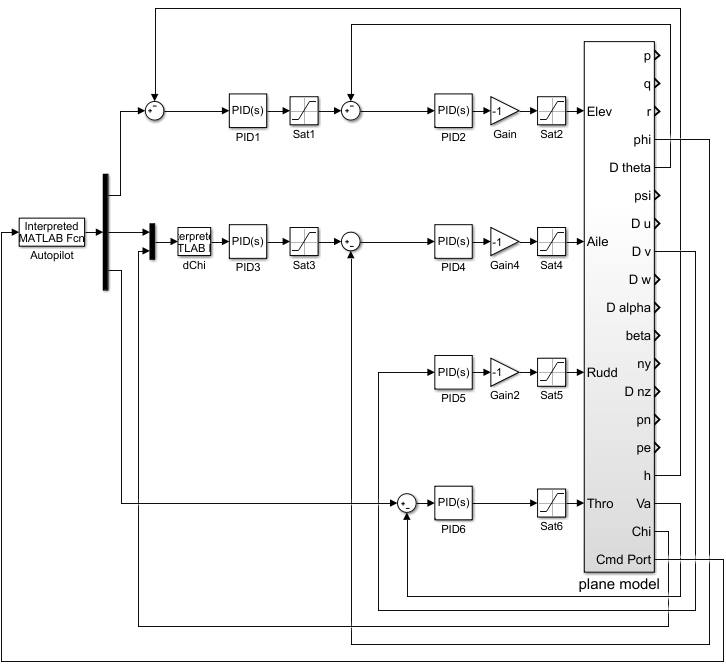
\includegraphics[width=\textwidth]{sim.png}
\caption{仿真系统模型}
\label{sim}
\end{figure}
图中plane model模块为飞机的状态空间模型,Autopilot模块使用状态机,根据飞机的速度,高度和航向确定当前飞行阶段的期望值。
仿真结果如图所示。
\begin{figure}[!h]
\centering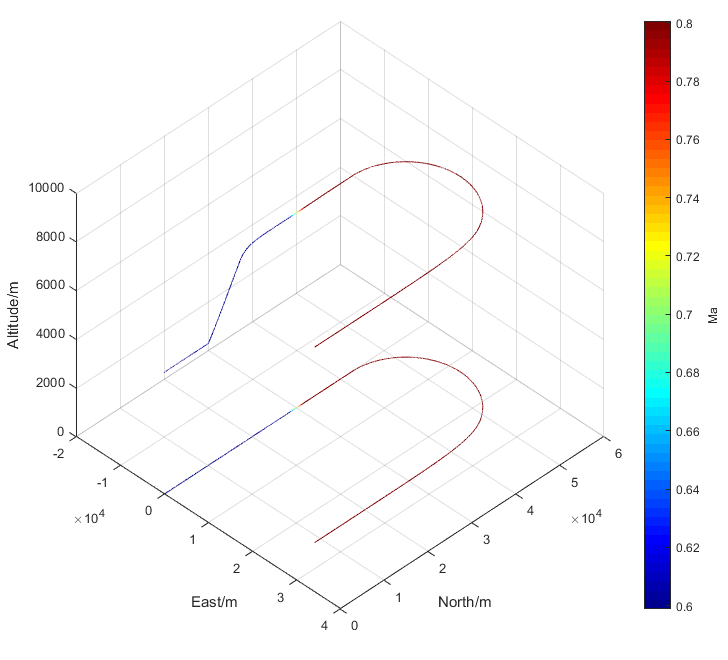
\includegraphics[width=\textwidth]{course.png}
\caption{飞机飞行航迹及其在水平面的投影}
\label{course}
\end{figure}

\begin{figure}[!h]
\centering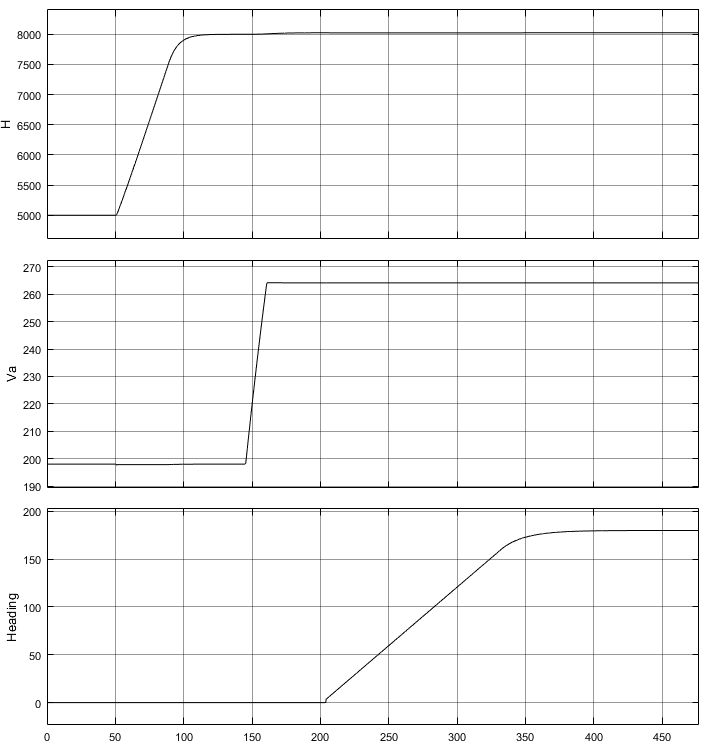
\includegraphics[width=\textwidth]{reshvh.png}
\caption{高度,速度,航向曲线}
\label{course}
\end{figure}

\begin{figure}[!h]
\centering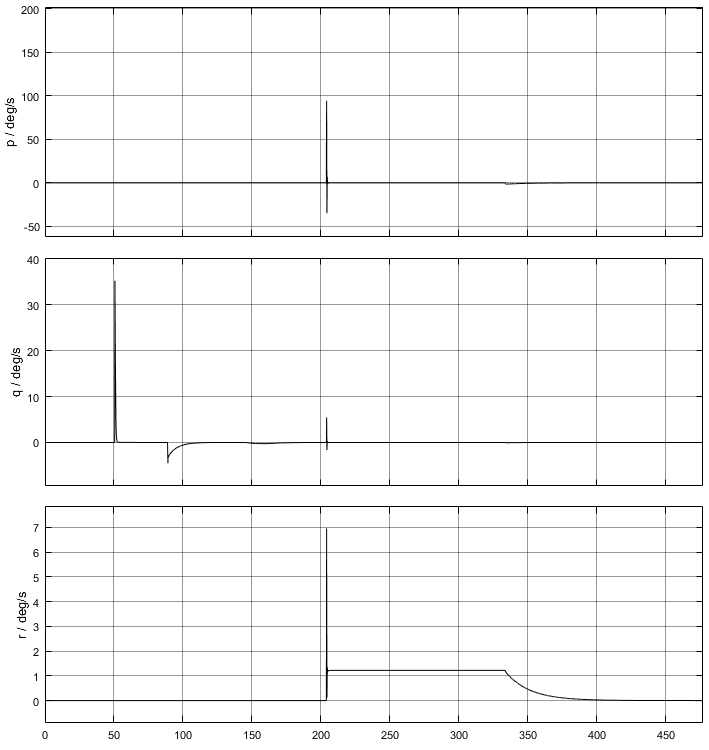
\includegraphics[width=\textwidth]{respqr.png}
\caption{体轴系角速率曲线}
\label{course}
\end{figure}

\begin{figure}[!h]
\centering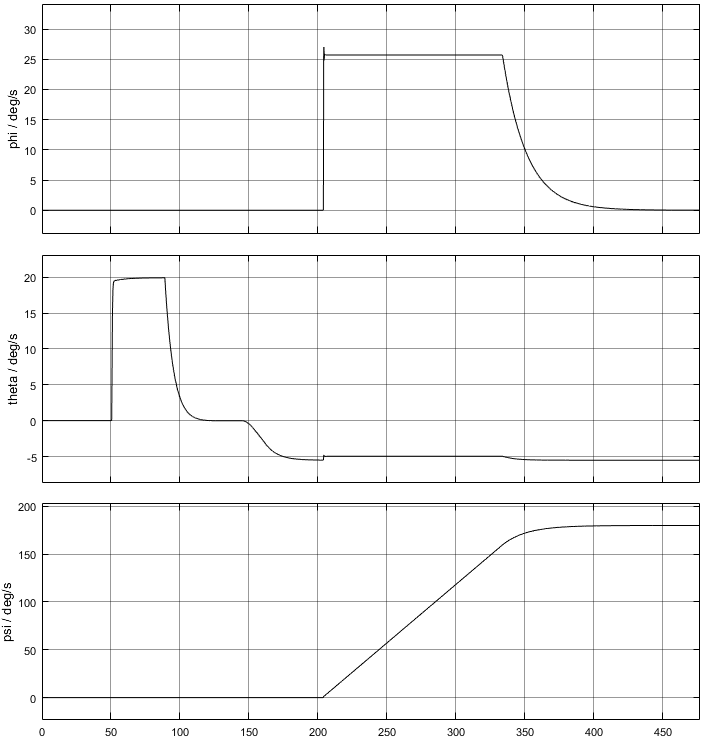
\includegraphics[width=\textwidth]{resptp.png}
\caption{姿态角曲线}
\label{course}
\end{figure}

\begin{figure}[!h]
\centering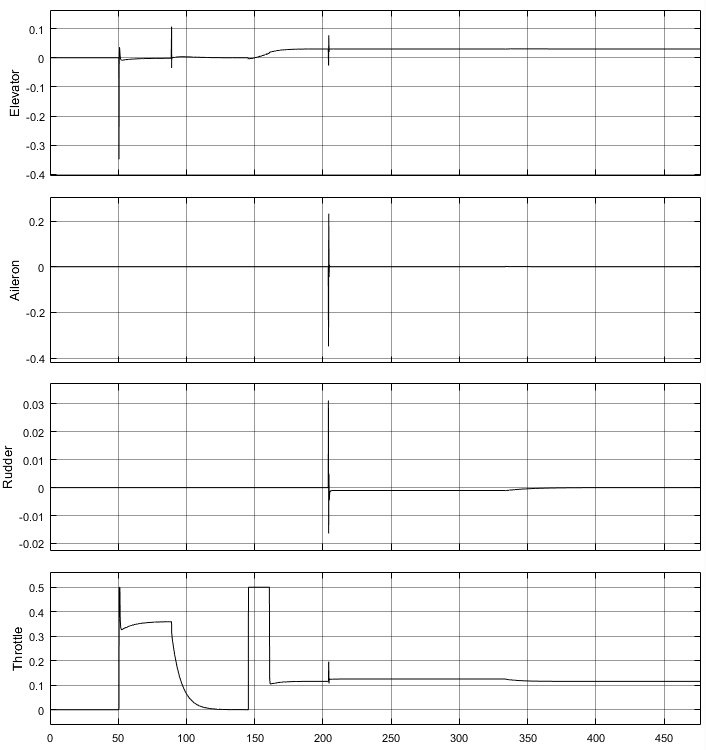
\includegraphics[width=\textwidth]{resctrl.png}
\caption{操纵量输出曲线}
\label{course}
\end{figure}
\section{Section 1}
\subsection{SubSection 1}
\subsubsection{SubSubsection 1}
\begin{figure}[!h]
\centering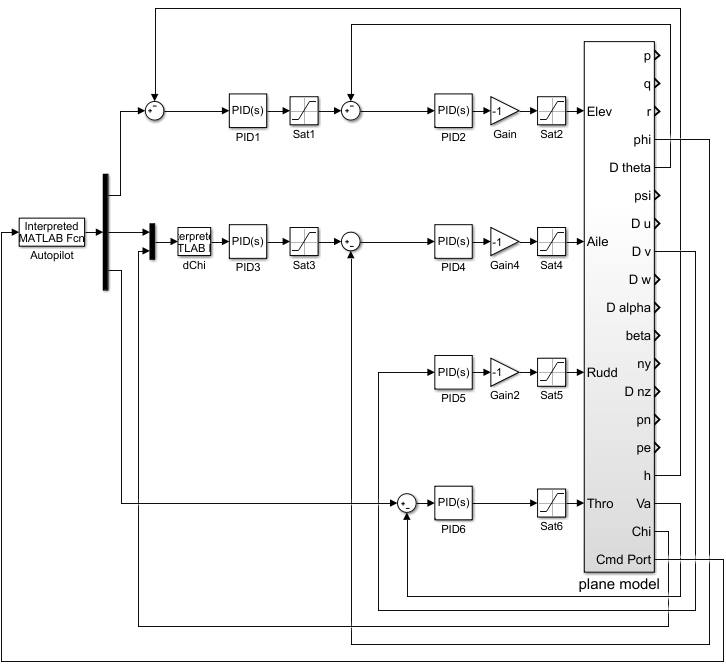
\includegraphics[width=\textwidth]{sim.png}
\caption{仿真系统模型}
\label{sim}
\end{figure}

\endinput
